\documentclass{article}
\usepackage[utf8]{inputenc}
\usepackage{comment}

\usepackage[margin=0.8in]{geometry}

\usepackage{tikz}
\usepackage{amsmath}
\usepackage{amsfonts}
\usetikzlibrary{arrows,automata}

\usepackage{graphicx}

\title{Automata Final}
\author{tyang27}
\date{May 2019}

\begin{document}

\maketitle

\section{Regular Languages}
\begin{comment}
\begin{itemize}
    \item $\Sigma$ - alphabet
    \item String over $\Sigma$ - finite sequence of symbols from alphabet
    \item $\varepsilon$ - empty string
    \item Language over $\Sigma$ - set of all possible strings over $\Sigma$
    \item Machine accepts string if consumes it and lands in a final state
    \begin{itemize}
        \item Let $w=w_1 w_2\dots w_n$
        \item M accepts $w$ if there is a sequence of states $r_1, r_2, \dots, r_n \in Q$ if:
        \item Valid start state - $r_0 = q_0$
        \item Valid transitions - $\delta(r_i, w_{i+1}) = r_{i+1}$
        \item Ends in final state - $r_n \in F$
    \end{itemize}
    \item Machine recognizes language $A$ if it accepts all strings in it, and does not accept any string outside of it, implies that $A$ is a regular language
    \item Union - $A \cup B = \{x | x \in A \textrm{ or } x \in B\}$
    \item Concatenation - $A \circ B = \{xy | x \in A, y \in B\}$
    \item Kleene star - $A^* = \{x_1x_2\dots x_k | k \geq 0, x_i \in A\}$
\end{itemize}
\end{comment}
\subsection{Deterministic Finite Automata}
$M = (Q, \Sigma, \delta, q_0, F)$
\begin{itemize}
    \item $Q$ = set of states
    \item $\Sigma$ = alphabet, set of symbols
    \item $\delta : Q \times \Sigma \rightarrow Q$ = transition function, maps states, symbols to new states
    \item $q_0 \in Q$ = start state
    \item $F \subseteq Q$ = set of final states
\end{itemize}

\subsection{Nondeterministic Finite Automata}
$M = (Q, \Sigma, \delta, q_0, F)$
\begin{itemize}
    \item $Q$ = states
    \item $\Sigma$ = alphabet
    \item $\delta : Q \times \Sigma_{\varepsilon} \rightarrow P(Q)$ = transition function, maps states, symbols/varepsilon to set of new states
    \item $q_0 \in Q$ = start state
    \item $F \subseteq Q$ = set of final states
\end{itemize}
Modified delta transition allows us to 1) varepsilon jump to states, 2) be at multiple states at once, and 3) have dead states

\subsection{Regular Expressions}
Base cases:
\begin{itemize}
    \item $a \in \Sigma$
    \item $\varepsilon$
    \item $\emptyset$
\end{itemize}
Operations:
\begin{itemize}
    \item $R_1 \cup R_2$
    \item $R_1 \circ R_2$
    \item $R_1^*$
\end{itemize}

\subsection{Converting between DFA/NFA/RE}

\subsubsection{DFA to NFA}
Trivial

\subsubsection{NFA to DFA}
Subset construction
\begin{itemize}
    \item $Q' = P(Q)$ - NFA states are subset of DFA states
    \item $\Sigma' = \Sigma$
    \item $\delta'(R, a) = \bigcup_{r \in R} E(\delta(r, a))$ if $R \in Q'$ - For each NFA state (a subset), we follow the DFA transition of each element in the set (a new subset). Apply varepsilon transition to the result of original transition.
    \item $q_0' = E(\{q_0\})$
    \item $F' = \{R \in Q' | \exists r \in R, r \in F\}$ - Final NFA states contain some original final state
\end{itemize}

\subsubsection{NFA to RE}
Ripping method using GNFA.

\begin{enumerate}
    \item Add new start state that varepsilon jumps to original start state
    \item Add new final state that all original final states varepsilon jump to 
    \item Replace commas with unions
    \item \begin{minipage}[t]{\linewidth}
    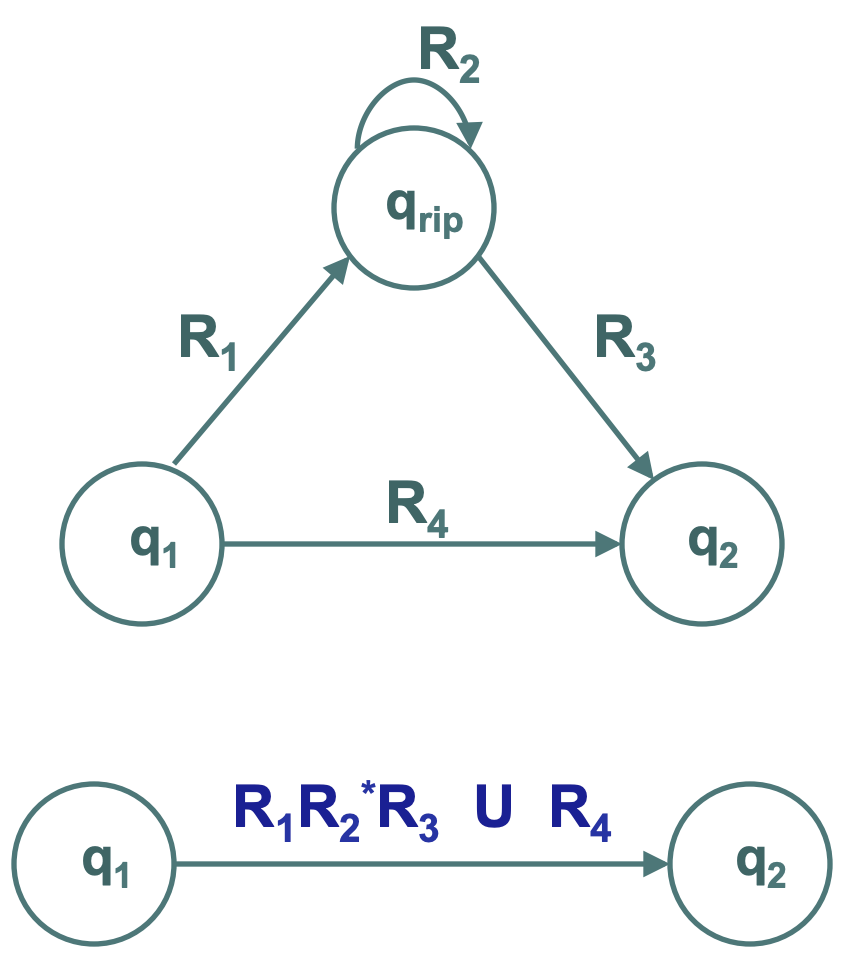
\includegraphics[scale=0.25]{rip.png}
    \end{minipage}
    \item Rip rip rip! Enumerate paths that go through $q_{rip}$ and link the two connections using the formula above.
\end{enumerate}

\subsubsection{RE to NFA}
Use process similar to induction.

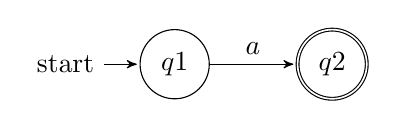
\begin{tikzpicture}[->,>=stealth',shorten >=1pt,auto,node distance=2cm,
        scale = 1,transform shape]

  \node[state,initial] (q1) {$q1$};
  \node[state,accepting] (q2) [right of=q1] {$q2$};
  \path (q1) edge              node {$a$} (q2);
\end{tikzpicture}

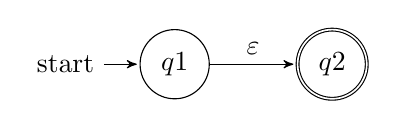
\begin{tikzpicture}[->,>=stealth',shorten >=1pt,auto,node distance=2cm,
        scale = 1,transform shape]
  \node[state,initial] (q1) {$q1$};
  \node[state,accepting] (q2) [right of=q1] {$q2$};

  \path (q1) edge              node {$\varepsilon$} (q2);
\end{tikzpicture}

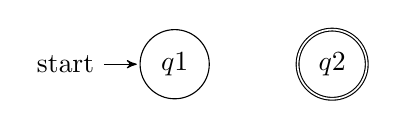
\begin{tikzpicture}[->,>=stealth',shorten >=1pt,auto,node distance=2cm,
        scale = 1,transform shape]

  \node[state,initial] (q1) {$q1$};
  \node[state,accepting] (q2) [right of=q1] {$q2$};
\end{tikzpicture}

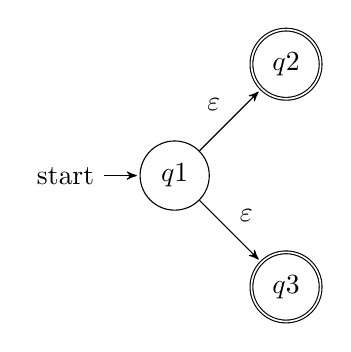
\begin{tikzpicture}[->,>=stealth',shorten >=1pt,auto,node distance=2cm,
        scale = 1,transform shape]
  \node[state,initial] (q1) {$q1$};
  \node[state,accepting] (q2) [above right of=q1] {$q2$};
  \node[state,accepting] (q3) [below right of=q1] {$q3$};

  \path (q1) edge              node {$\varepsilon$} (q2)
        (q1) edge              node {$\varepsilon$} (q3);
\end{tikzpicture}

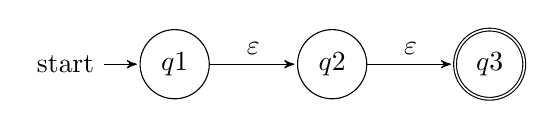
\begin{tikzpicture}[->,>=stealth',shorten >=1pt,auto,node distance=2cm,
        scale = 1,transform shape]
  \node[state,initial] (q1) {$q1$};
  \node[state] (q2) [right of=q1] {$q2$};
  \node[state,accepting] (q3) [right of=q2] {$q3$};

  \path (q1) edge              node {$\varepsilon$} (q2)
        (q2) edge              node {$\varepsilon$} (q3);
\end{tikzpicture}

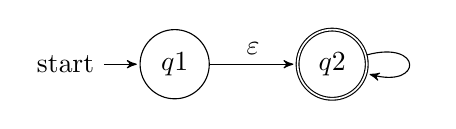
\begin{tikzpicture}[->,>=stealth',shorten >=1pt,auto,node distance=2cm,
        scale = 1,transform shape]
  \node[state,initial] (q1) {$q1$};
  \node[state,accepting] (q2) [right of=q1] {$q2$};

  \path (q1) edge              node {$\varepsilon$} (q2)
        (q2) edge[loop right]              node {} (q2);
\end{tikzpicture}

\subsection{Closure}
\subsubsection{Union using NFA}
\begin{itemize}
    \item $Q = Q_1 \cup Q_2 \cup \{q_{new}\}$
    \item $\Sigma = \Sigma_1 = \Sigma_2$
    \item $\delta(r,a)$ = 
    $\begin{cases}
    \delta_1(r,a) & \textrm{ if } r \in Q_1\\
    \delta_2(r,a) & \textrm{ if } r \in Q_2\\
    \{q_{01}, q_{02}\} & \textrm{ if } r = q_{new}, a = \varepsilon\\
    \emptyset & \textrm{ if } r=q_{new}, a \neq \varepsilon
    \end{cases}$
    \item $q_0 = q_{new}$
    \item $F = F_1 \cup F_2$
\end{itemize}

\subsection{Pumping Lemma}
\subsubsection{Formal}
If $A$ is a regular language, then there exists an integer $p$ where if $s$ from $A$ is any string of length at least $p$, then $s$ may be divided into three pieces, $s=xyz$, such that:
\begin{itemize}
    \item $\forall i \geq 0$, $xy^{i}z \in A$.
    \item $|y| > 0$
    \item $|xy| \leq p$
\end{itemize}
\subsubsection{Informal}
Given a regular language $A$, the pumping lemma holds. The pumping lemma says that if we have a long string (a string with length greater than the number of states), we know that there must be some loop in the machine, and we can partition the machine into three pieces, $xyz$, where y is the loop.
\begin{itemize}
    \item If we pump the loop 0 or more times, it is still in the language.
    \item The loop exists, in the sense that it has at least one state.
    \item The leadup to the loop and the loop combined fit into the machine.
\end{itemize}

\subsection{Proving nonregularity}
FSOC, assume that $A$ is regular. Then, the properties of pumping lemma apply, enumerate. Consider a long string $s=xyz$ (choose $s$) with an arbitrary partition up to $p$ that satisfies pumping lemma. If we pump it more or less (choose $i$), then it is no longer in the language.

\subsection{Other notes}
\begin{itemize}
    \item To show that reversed strings are closed under regular languages, we can just swap the arrows in a DFA, but cannot do so in NFA. This is because NFA has dead states.
\end{itemize}


\section{Context Free Languages}
\subsection{Properties}
\begin{itemize}
    %\item Consistency - generates all strings in language.
    %\item Consistency - generates only strings in language.
    \item Ambiguous - string derived from grammar in fundamentally different ways. Show that either 1) give different parse trees or 2) different leftmost derivations.
\end{itemize}

\subsection{Context Free Grammar}
$G = (V, \Sigma, R, S)$
\begin{itemize}
    \item $V$ - variables, finite set of symbols, typically caps
    \item $\Sigma$ - terminals, finite set of symbols, disjoint from variables ($V \cap \Sigma = \emptyset$), typically lowercase
    \item $R$ - finite set of rules, e.g. $A \to B$
    \item $S \in V$ - start symbol
\end{itemize}
Start with $S$, derive by repeating rules until no more variables, only terminals.

\begin{comment}
\subsubsection{Parse Tree}
\begin{itemize}
    \item Leaves are terminals.
    \item Internal nodes are variables.
    \item Branches correspond to concatenation
\end{itemize}
\end{comment}

\subsubsection{Chomsky Normal Form}
Equivalent to CFG. Basically, CFG with certain conditions. $2n-1$ to derive a string of $n$. Conditions:
\begin{itemize}
    \item $A \to BC$
    \item $A \to a$
    \item $B,C$ cannot be $S$
    \item Only $S$ can go to $\varepsilon$
\end{itemize}

\subsection{Converting from RE to CFG}
\begin{itemize}
    \item $a = S \to a$
    \item $\varepsilon = S \to \varepsilon$
    \item $\emptyset = S \to S$
    \item $R_1 \cup R_2 = S \to S_1 | S_2$
    \item $R_1 \circ R_2 = S \to S_1 S_2$
    \item $R_1^* = S \to S_1 S$
\end{itemize}

\subsection{Push Down Automata}
$P = (Q, \Sigma, \Gamma, \delta, q_0, F)$
\begin{itemize}
    \item $Q$ = finite set of states
    \item $\Sigma$ = alphabet, finite set of symbols
    \item $\Gamma$ = stack alphabet, finite set of symbols
    \item $\delta: Q \times \Sigma_{\varepsilon} \times \Gamma_{\varepsilon} \to P(Q\times \Gamma_{\varepsilon})$ = transition function, e.g. $a, b\to c$
    \item $q_0$ = start state
    \item $F \subseteq Q$ = set of final states
\end{itemize}
\subsubsection{Useful transitions}
\begin{itemize}
    \item $\textrm{symbol } a, \textrm{ pop } b \to \textrm{push } c$ = take arrow if symbol in string is $a$ and top of stack is $b$. Pop $b$ off stack and push $c$.
    \item $a, \varepsilon \to \varepsilon$ = consume symbol, ignore stack
    \item $\varepsilon, \varepsilon \to b$ = consume no symbol, push onto stack
    \item $\varepsilon, b \to \varepsilon$ = consume no symbol, pop off of stack
    \item $\varepsilon, \varepsilon \to \varepsilon$ = consume no symbol, ignore stack
\end{itemize}

\subsection{Converting from CFG to PDA}
\begin{itemize}
    \item The general idea is that we place an empty marker on the stack and on top of that, the reverse of all possible generations. We put rules that consume the input $x, x\to \varepsilon$ to check if we can uncover the $\$$, meaning that it is a valid string.
    
    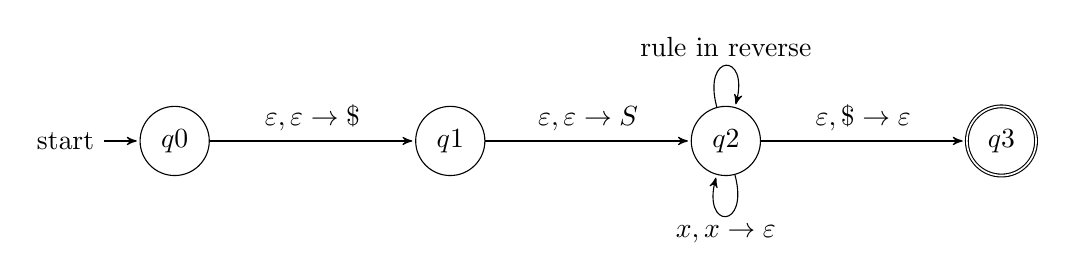
\begin{tikzpicture}[->,>=stealth',shorten >=1pt,auto,node distance=3.5cm,
        scale = 1,transform shape]

  \node[state,initial] (q0) {$q0$};
  \node[state] (q1) [right of=q0] {$q1$};
  \node[state] (q2) [right of=q1] {$q2$};
  \node[state,accepting] (q3) [right of=q2] {$q3$};

  \path (q0) edge              node {$\varepsilon, \varepsilon \to \$$} (q1)
        (q1) edge              node {$\varepsilon, \varepsilon \to S$} (q2)
        (q2) edge[loop above]              node {$\textrm{rule in reverse}$} (q2)
        (q2) edge              node {$\varepsilon, \$ \to \varepsilon$} (q3)
        (q2) edge[loop below]              node {$x, x \to \varepsilon$} (q2);

\end{tikzpicture}
\end{itemize}

\subsection{Converting from PDA to CFG}
A bit too involved, but know that it is possible.

\subsection{Other notes}
\begin{itemize}
    \item Stacks lack notion of emptiness, so often use \$ symbol emptiness\\
    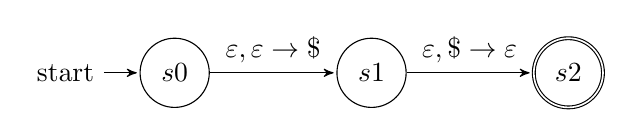
\begin{tikzpicture}[->,>=stealth',shorten >=1pt,auto,node distance=2.5cm,
        scale = 1,transform shape]

  \node[state,initial] (s0) {$s0$};
  \node[state] (s1) [right of=s0] {$s1$};
  \node[state,accepting] (s2) [right of=s1] {$s2$};

  \path (s0) edge              node {$\varepsilon, \varepsilon\to \$$} (s1)
        (s1) edge              node {$\varepsilon, \$ \to \varepsilon$} (s2);

\end{tikzpicture}
\end{itemize}

%===================================%
% mid 2
%===================================%
\section{Context-free languages}
\subsection{Pumping lemma for context-free languages}
If $A$ is a context-free language, then $\exists p$, the pumping length. If $s$ is a long string in A ($s \in A$ and $|s| > p$), then $s$ may be divided into five pieces $s=uvxyz$ s.t.
\begin{itemize}
    \item $\forall i \geq 0,uv^i xy^i z \in A$
    \item $|vy|>0$ (note, $v$ or $y$ can be the empty string, but not both)
    \item $|vxy| \leq p$
\end{itemize}
If a string of terminals is longer than the number of rules in Chomsky Normal form (informally), we know that a variable is repeated, and we can replace the variable inside with the one outside recursively. Pumping once, we get $uvvxyyz$.

\subsection{Showing nonCFLarity}
Assume, FSOC, that $A$ is a CFL. Let $p$ be the pumping length given by PL for CFLs. Consider a string $s=uvxyz$ (e.g. $s=a^p b^p c^p \in A$) with at least length $p$. State some property about what $v$ and $y$ could be (e.g. we know that $xyz$ cannot contain more than two different types of symbols). Pump up, so the number of occurrences of at least one of the symbols is not changing, meaning that the number of occurrences of one type of symbol is still $p$, while the number of occurences of the other symbol is now $p+k$ for some $k$.

\subsection{Closure}
\begin{itemize}
    \item Regular operators: union, concatenation, kleene star, intersection, complement
    \item Context free operators: union, concatenation, kleene star
    \item Turing decidable: union, intersection, concatenation, complement, and kleene star
    \item Turing recognizable: union, intersection, concatenation, and kleene star
\end{itemize}

\section{Turing Machines}
\subsection{Church Turing Thesis}
\begin{itemize}
    \item Algorithms and turing machines are basically equivalent.
\end{itemize}
\subsection{Showing Turing Decidable}
\begin{itemize}
    \item Guaranteed to halt on accept/reject.
    \item By given, want, construction, correctness. Make sure that our machine terminates.
\end{itemize}

\subsection{Showing Turing Recognizable}
\begin{itemize}
    \item Guaranteed to accept, but may loop.
    \item By given, want, construction, correctness.
    \item Make sure that inner loops terminates in finite steps, but outer loop can be infinite. E.g. use shortlex ordering up to a certain amount of steps.
\end{itemize}

\subsection{Co-Turing Recognizable}
\begin{itemize}
    \item The complement is Turing Recognizable.
    \item If Co-TR and TR, then TD.
\end{itemize}

%===================================%
% mid 3
%===================================%

\section{Undecidable languages}
\begin{itemize}
    \item $A_{TM} = \{\langle M, w\rangle | M \textrm{ is a TM and } M(w) \textrm{ accepts} \}$, TR, but not co-TR
    \item $HALT_{TM} = \{\langle M, w\rangle | M \textrm { is a TM and } M(w) \textrm{ halts}\}$
    \item $EMPTY_{TM} = \{\langle M \rangle | M \textrm{ is a TM and } L(M)=\emptyset\}$
\end{itemize}

\section{Reduction}
\begin{itemize}
    \item $A\leq_m B$: If $B$ is decidable, then $A$ is decidable. If $A$ is undecidable, then $B$ is also undecidable.
    \item $A_{TM} \leq_m HALT_{TM}$: FSOC, assume that the halting problem is decidable by $D_{HALT}$. Then we can use that to create $A_{TM}$. Run $D_{HALT}$ on $M_{IN}$. If it halts, reject. Otherwise, run $M_{IN}$ on $w_{IN}$. However, we know that $A_{TM}$ is undecidable, so $HALT_{TM}$ must also be undecidable.
    \item $EMPTY_{TM} \leq_m A_{TM}$: FSOC, say that the emptiness problem is decidable by $D_{EMPTY}$. Then we can use that to create $A_{TM}$. Construct a new machine such that if the string is not $w_{IN}$, reject. Otherwise, run $M_{IN}(w_{IN})$ and output what it outputs. Then, if the emptiness decider accepts, we know that the machine does not accept the string or the string is not correct. If it rejects, there must be a single item in it, so we know that set is not empty, so it must accept a string.
    \item $ALL_{CFG} \leq_m EQUAL_{CFG}$: FSOC, say that the emptiness problem is decidable by $D_{EQUAL}$. Then, we can use that to create $EQUAL_{CFG}$. We construct a CFG that accepts everything. If we run $D_{EQUAL}$ on our constructed CFG and $G_{IN}$, and it accepts, we know that $G_{IN}$ accepts everything.
    \item $ALL_{CFG}\leq_m \{\langle G_1, G_2\rangle | \textrm { are CFGs and } L(G_1)=\overline{L(G_2)}\}$: Similar to above. Instead, we construct a CFG that accepts nothing as our $G_2$, and if the decider accepts, we know that it accepts everything
    \item $A_{TM} \leq_m REG_{TM}$: Create a machine that runs $M(w)$. If it accepts, accept nonregular strings of the form $0^{n}1^{n}$, otherwise reject everything. Then, if we run $REG_{TM}$, deciding regularity also tells us if $w$ was accepted, since we know that if $M(w)$ accepts, the language is nonregular, and if $M(w)$ rejects, we would have an empty set, which we know is regular.
    \item The way that you want to think about this is, if A reduces to B, FSOC, say that we have a decider D for B. How can we create a machine that produces a language that could be used on D to answer A?
\end{itemize}
\subsection{Template for $A \leq_m B$}
\begin{itemize}
    \item Say that we know that $A$ is unTD
    \item FSOC, say that we have a TM decider $D$ that decides B.
    \item Want a construction for TM $L$ that answers $A$ s.t. if input is in $A$, $L$ accepts, else $L$ rejects
    \item Construct inner TM $I$ where on input $x$, may or may not ignore x or w to create a set that is compliant with $B$ and answers $A$. For $A_{TM}$, we can create a set based on $I(w)$'s output, since we never even run the machine. Run D on $I$.
    \item Correctness by looking at the properties of the language produced and seeing that if an input is in $A$, then our machine $I$ will accept. If an input is not in $A$, then our machine $I$ will reject.
    \item However, $D$ does not exist, so we have reached a contradiction.
    \item Synonymous for TR
\end{itemize}

\section{Mapping Reduction}
\begin{itemize}
    \item $A\leq_m B$, $f:\Sigma^*\to \Sigma^*$ s.t. $w \in A$ iff $f(w) \in B$
    \item If $A\leq_m B$ and $B$ is TD/TR, then $A$ is TD/TR ($B$ is a harder problem and you can solve $B$)
    \item If $A\leq_m B$ and $A$ is not TD/TR, then $B$ is not TD/TR
    \item Similar in spirit to the normal reduction template, just output your input instead of pretending there's a decider and running it.
\end{itemize}
\section{Complexity and P and NP}
\begin{itemize}
    \item Every multitape $T(n)$ has an equivalent $O(T(n)^2)$ single tape.
    \item Every $T(n)$ nondeterministic has an equivalent $O(2^{T(n)})$
    \item P: polynomial in deterministic single tape
    \item NP: polynomial in nondeterministic single tape, or verifiable in polynomial time
\end{itemize}


\end{document}
